\capitulo{4}{Aplicación web para la detección de movimientos involuntarios}

\section{Objetivo}

La aplicación \textbf{InvoluntTrack}, desarrollada en formato web, permite evaluar la capacidad del usuario para seguir una trayectoria lineal predefinida mediante el cursor del ratón. En condiciones normales, cuando el sistema nervioso motor funciona correctamente, el usuario es capaz de mantener el cursor dentro de los límites a lo largo de todo el recorrido. Por el contrario, si existe alguna lesión en el sistema nervioso que provoque la alteración del movimiento, se producirán desviaciones del cursor respecto a la trayectoria. La aplicación detecta y registra estas salidas, interpretándolas como posibles movimientos involuntarios.

El programa no pretende ser una herramienta de diagnóstico, sino un apoyo a la toma de decisiones clínicas permitiendo detectar patrones de movilidad involuntaria de forma rápida y visual.

El nombre de la aplicación surge de la combinación de dos conceptos. Por un lado, \textbf{"Involunt"}, abreviatura de involuntario, representando al tipo de movimientos que la aplicación pretende detectar. Por otro lado, \textbf{"Track"}, haciendo referencia a la trayectoria que realiza el usuario durante la prueba.
\clearpage
\section{Funcionamiento}
Al comenzar la prueba, aparece una trayectoria predefinida sobre un recuadro interactivo, con un punto de inicio y un punto de fin definidos. El usuario debe desplazar el cursor del ratón desde el inicio hasta el fin intentando mantenerlo dentro del tramo. Durante el recorrido, la aplicación detecta cualquier desviación, marcando y registrando los puntos donde se han producido las salidas. Al finalizar, se muestra un resumen de las salidas detectadas y una clasificación orientativa, además tiene la posibilidad de guardar la imagen que incluye tanto la trayectoria original como la seguida por el usuario, para posteriores análisis o elaboración de informes.

La aplicación tiene disponibles cuatro niveles de dificultad en función de la complejidad que se requiera para el usuario, desde una línea horizontal en el nivel más sencillo, hasta trayectorias con curvas y cambios bruscos de movimientos en los niveles más complejos. Esto permite adaptar la prueba a distintos perfiles en función del nivel de afectación del sistema nervioso.

\begin{center}
	    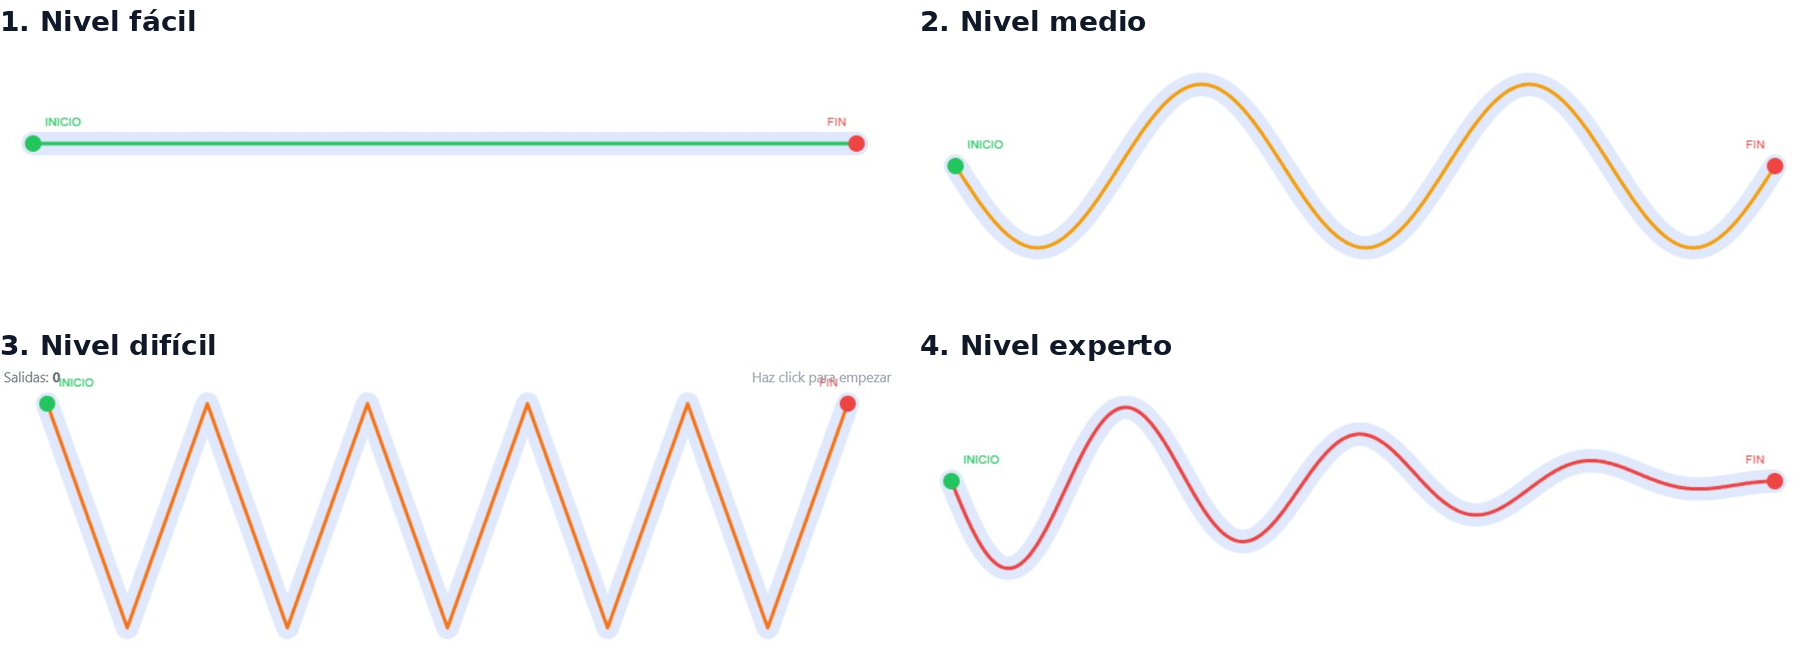
\includegraphics[width=1\textwidth]{img/niveles.png}
	    \captionof{figure}{Niveles disponibles en la aplicación.}
	    \label{fig:niveles}
	\end{center}

Además, la aplicación cuenta con un parámetro de tolerancia de error configurable por el usuario. Este parámetro, definido en pixeles, establece un margen de error alrededor de la trayectoria, funcionando como el límite máximo. Es decir, hasta que el usuario no traspasa el margen de error con el cursor, la aplicación no registra la salida. La tolerancia al igual que los niveles de dificultad, permite personalizar la prueba a cada usuario.
\clearpage
\section{Código}

La aplicación se ha desarrollado a través de Streamlit, aunque el funcionamiento central se encuentra en un bloque de HTML y JavaScript, contando principalmente con las siguientes funciones:


La función \textbf{buildPath()}, es la encargada de crear la trayectoria que el usuario debe seguir. Para ello, crea 500 puntos a lo largo del recuadro y según el nivel de dificultad seleccionado, varía la altura de cada punto para formar un tipo de línea u otro. 

En el caso de dificultad fácil, todos los puntos tienen la misma altura consiguiendo una línea recta, mientras que en los casos mas complejos se utilizan funciones matemáticas, como los senos para conseguir trayectorias con forma de ondas.

La función \textbf{ndist()} calcula la distancia mínima entre la posición del cursor y la trayectoria predefinida. Para ello, recorre los puntos que definen el camino y calcula la distancia de todos los puntos con el cursor y selecciona la menor, de esta forma el programa sabe dónde se encuentra el cursor durante el recorrido. 

La posición del cursor, se utiliza para determinar si el cursor se encuentra dentro o fuera de los límites, mediante la función \textbf{updateTrace()}. Esta función, compara la posición del cursor con el valor de tolerancia establecido. Si la posición es mayor que la tolerancia: se considera fuera, marca el punto de salida y registra la desviación en el contador de salidas. En caso contrario, la aplicación continua con el recorrido normal.

Es importante destacar que la aplicación registra solamente la primera salida de la trayectoria. Si el usuario se encuentra fuera del recorrido, no se contabilizan nuevas salidas hasta que el cursor vuelva a entrar dentro de los límites de la trayectoria y lo vuelva a superar. De esta forma, se tiene un recuento de las salidas y no del tiempo que el usuario pasa fuera.

Las funciones \textbf{startTrace()} y \textbf{finishTrace()}, se encargan del inicio y el final de la prueba. Cuando el usuario hace click en el recuadro, comienza a dibujar la trayectoria del cursor, hasta llegar al punto de fin, donde la prueba finaliza automáticamente. Cuando llega a este punto, también se desbloquean las opciones de ver resultados, guardar imagen o reiniciar prueba.

 La función \textbf{draw()} se encarga de la visualización de la prueba. Permite representar la trayectoria guía, la trayectoria del cursor del usuario, el margen de error de la tolerancia, así como los puntos donde el cursor supera los límites.

Por último, entre las funciones principales se encuentra \textbf{showResults()} que genera una interpretación orientativa en función del número de salidas:
	\begin{itemize}
	\item Número de salidas = 0 -> No hay movimientos involuntarios
	\item Número de salidas < 10 -> Posible afectación
	\item Número de salidas > 10 -> Afectación considerable
	\end{itemize}
	
Además cuenta con otras funciones como \textbf{saveImage()} que permite guardar la imagen con la trayectoria guía y la trayectoria generada por el usuario, o la función \textbf{resetCanvas()} que borra las trayectorias creadas y reinicia los contadores y resultados, permitiendo repetir la prueba.

\section{Interfaz}

La aplicación cuenta con una pantalla principal donde aparecen los siguientes elementos:

\subsection{Selección del nivel de dificultad:}
El usuario o personal médico responsable de realizar la prueba puede elegir a través de un desplegable el nivel de dificultad, en función de las características del usuario.

\begin{center}
	    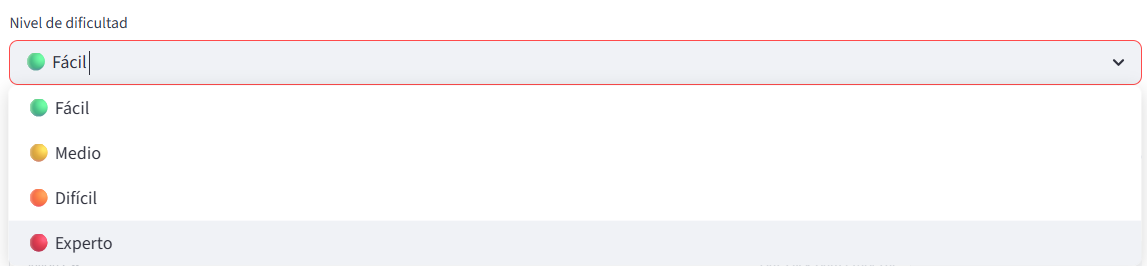
\includegraphics[width=0.9\textwidth]{img/nivel_dificultad.png}
	    \captionof{figure}{Selección de niveles de dificultad.}
	    \label{fig:selección_niveles}
	\end{center}
	
\subsection{Ajuste de tolerancia:}
La tolerancia se puede ajustar deslizando el indicador sobre la siguiente barra hasta obtener el valor correspondiente. Por defecto, todos los niveles tienen un nivel de tolerancia de 10 pixeles.

\begin{center}
	    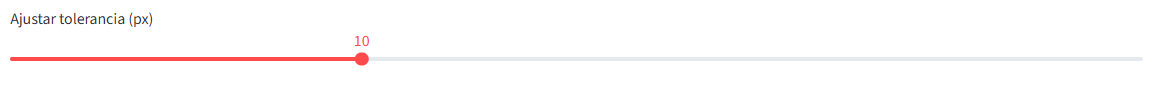
\includegraphics[width=1\textwidth]{img/tolerancia.png}
	    \captionof{figure}{Ajuste de tolerancia.}
	    \label{fig:selección_niveles}
	\end{center}
	
\subsection{Recuadro interactivo:}
Este recuadro permite al usuario dibujar la trayectoria guiándose del patrón predefinido. Cuando el usuario sobrepasa los límites establecido, la aplicación marca con un punto las zonas de salidas e incrementa el contador, obteniendo el número de desviaciones total.

\begin{center}
	    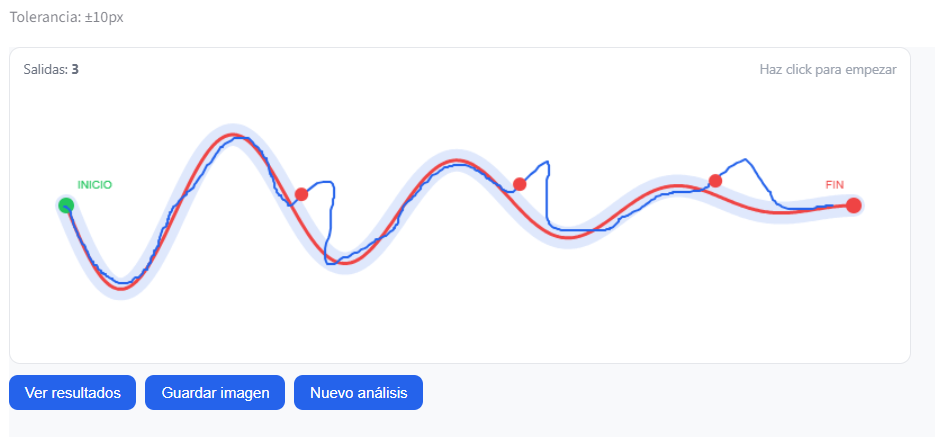
\includegraphics[width=0.55\textwidth]{img/prueba_trayectoria.png}
	    \captionof{figure}{Ejemplo de trayectoria (usuario).}
	    \label{fig:ejemplotrayectoria}
	\end{center}
	
Cuando el usuario llega al final de la trayectoria definida, aparecen tres botones que permiten:

\begin{itemize}
\item Ver los resultados de la prueba. Principalmente son estimaciones que pueden ayudar al diagnóstico, por lo que el personal médico que realice la prueba es el encargado de interpretarlos y considerar si son válidos para el diagnóstico final:

\begin{center}
	    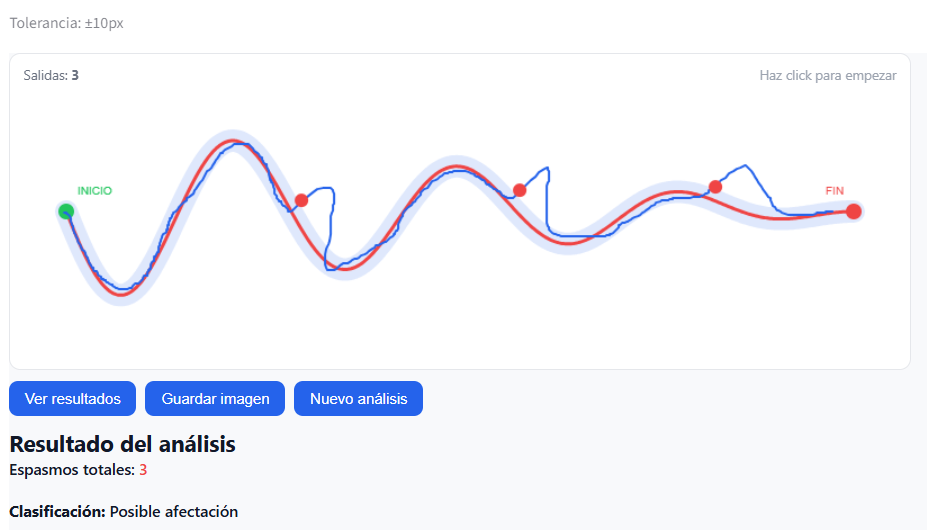
\includegraphics[width=0.7\textwidth]{img/resultados.png}
	    \captionof{figure}{Resultados de ejemplo.}
	    \label{fig:resultados}
	\end{center}

\item Guardar la imagen de la trayectoria realizada por el usuario junto a la trayectoria guía:
\begin{center}
	    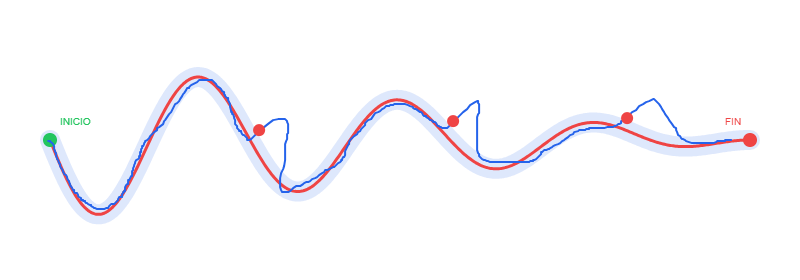
\includegraphics[width=0.7\textwidth]{img/trayectoria_guardada.png}
	    \captionof{figure}{Trayectoria guardada.}
	    \label{fig:guardado}
	\end{center}

\item Por último, reiniciar la prueba, limpiando las trayectorias realizadas y poniendo a cero todos los contadores

\subsection{Interfaz global:}

\begin{center}
	    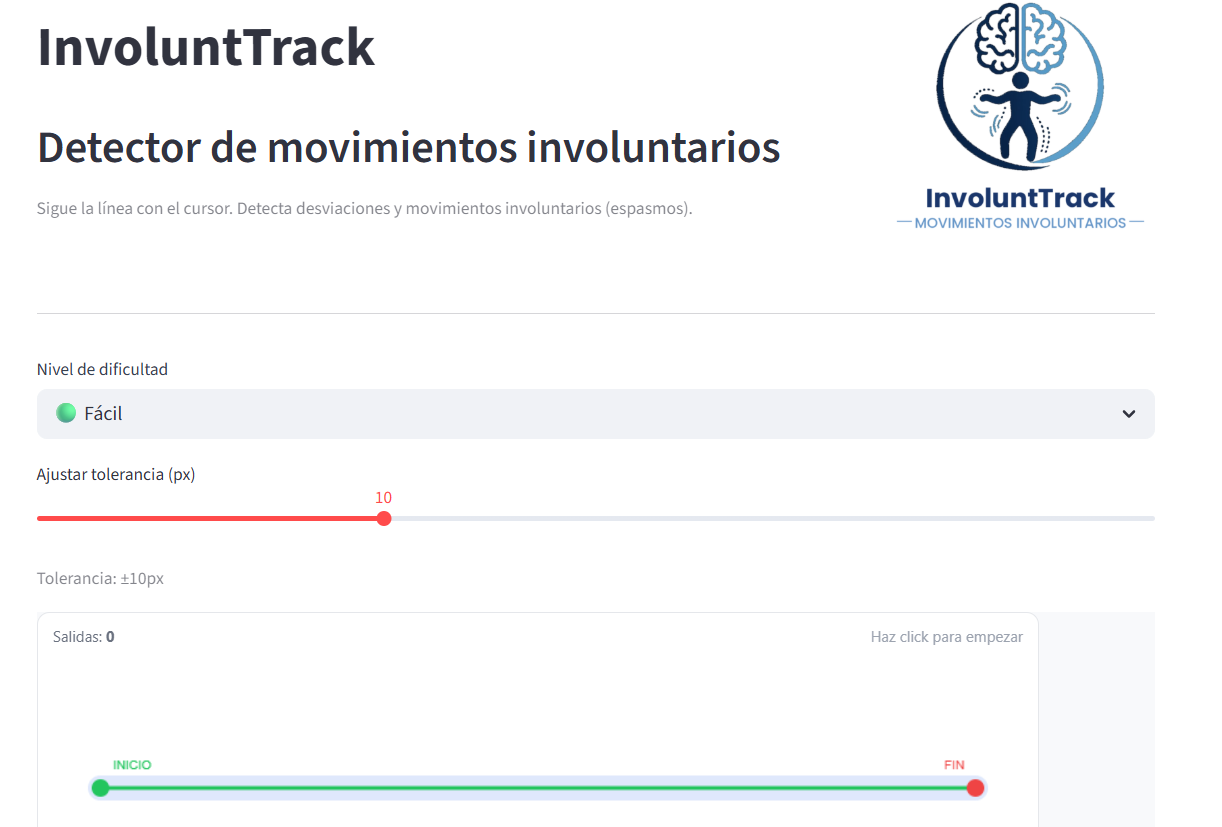
\includegraphics[width=1\textwidth]{img/interfaz_global.png}
	    \captionof{figure}{Interfaz global.}
	    \label{fig:interfaz}
	\end{center}

\end{itemize}

\clearpage
\section{Posibles mejoras}

La aplicación desarrollada es un prototipo funcional cuyo objetivo es demostrar el funcionamiento del programa propuesto para la detección de movimientos involuntarios. Por este motivo, presenta aspectos que pueden ser mejorados para aumentar la precisión, funcionalidad y accesibilidad.

\begin{itemize}
\item Emplear distintos sistemas de entrada, como pantallas táctiles o tablets, que permitan simular situaciones de movimiento más realistas y faciliten la adaptabilidad a usuarios que no puedan manejar el ratón.
\item Crear trayectorias más complejas y aleatorias para que los usuarios no se adapten a los mismos recorridos
\item Implementar nuevas pruebas que permitan detectar otros tipos de afectaciones neurológicas.
\item Incorporar nuevas métricas como velocidad del cursor, cambios bruscos de dirección o intensidad de temblor.
\item Utilizar clasificaciones más representativas, validadas por expertos neurológicos.
\item Añadir un sistema de usuarios que permita guardar la información de distintos pacientes, las pruebas realizadas, informes, trayectorias ...

\end{itemize}

\section{Presupuesto}

El presupuesto aproximado para el desarrollo de la aplicación web se ha calculado teniendo en cuenta tanto la parte hardware como software necesarias, así como el coste asociado al trabajo del personal técnico.

En cuanto al hardware, ha sido necesario principalmente un equipo informático ya sea portátil o de sobremesa, incluyendo sistemas de entrada de información claves para el funcionamiento de la aplicación como el ratón del ordenador.
\clearpage
\begin{itemize}
\item \textbf{Ordenador portátil:} se toma como referencia el modelo de portátil utilizado durante el desarrollo del trabajo. Consiste en un ordenador HP con procesador \textit{intel core i7} y dispone de la versión \textit{windows 11}, cuyo precio ronda los 780 € \cite{hp_15_fd0334ns_pccomponentes}. Aunque existen otras opciones más económicas igualmente válidas.
\item \textbf{Ratón (mouse):} los precios de estos dispositivos rondan en torno a los 10-13€ \cite{conceptronic_regas_tw5_pccomponentes}, por lo que esta decisión dependerá del usuario que vaya a utilizar la aplicación siempre y cuando sea funcional.
\end{itemize}

Respecto a la parte software, la aplicación se ha desarrollado a través de la librería de Python Streamlit junto a otros lenguajes como JavaScript y HTML. Estas herramientas son de acceso libre y no requieren el uso de licencias de pago, por lo que esta parte del desarrollo no supone ningún coste económico adicional.

Por otro lado, se incluyen los costes personales que suponen el desarrollo de la aplicación, estimado en base al sueldo medio de un ingeniero biomédico/de la salud junior que ronda entre los 25000€ y 35000€ anuales \cite{ufv_biomedico_salario_espana}, lo que se traduce a aproxiamdamente 2000€-2500€ mensuales. Al tratarse de un proyecto desarrollado por un equipo de cuatro personas, este coste se ha tenido en cuenta considerando la colaboración conjunta de todos los integrantes del grupo, multiplicando este valor por cuatro.

\begin{table}[h]
\centering
\begin{tabular}{|l|l|l|}

\hline
\rowcolor{gray!20}
\textbf{Concepto} & \textbf{Descripción} & \textbf{Coste estimado} \\ \hline
Hardware & Ordenador portátil & 780 € aprox. \\ 
Hardware & Sistemas de entrada (ratón) & 13 € aprox. \\ \hline
Software & Streamlit, JavaScript, HTML (software libre) & 0 € \\ \hline
Personal (1 persona) & Ingeniero biomédico junior (mensual) & 2000 € -- 2500 € \\ 
Personal (4 personas) & Equipo de desarrollo (mensual) & 8000 € -- 10000 € \\ \hline
\rowcolor{yellow!30}
\textbf{Total estimado} &  & \textbf{8793 €} \\ \hline
\end{tabular}
\caption{Presupuesto del proyecto}
\label{tab:presupuesto}
\end{table}